\chapter{相关技术介绍}\label{chap:relate}

由于本系统涉及软硬件协同设计,在进行设计前需要对神经网络算法、RISC-V 处理器以及 FPGA 平台有足够的认识。在本系统的设计中,我们需要选择合适的神经网络算法,并对其进行硬件加速。由于不是所有的运算都适合放在 FPGA 上实现,同时也为了加速器通用性的考虑,本设计中还使用一个 RISC-V 处理器来分担一部分运算任务以及流程控制的工作。

\section{神经网络概述}

\subsection{卷积神经网络概述}

\begin{figure}[!htbp]
    \centering
    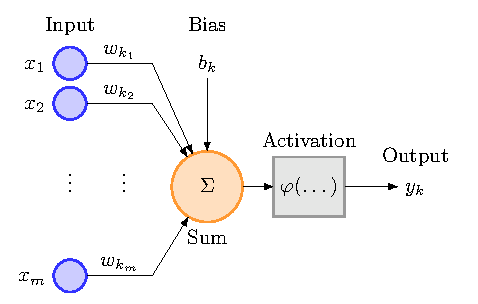
\includegraphics[width=0.5\textwidth]{neuron}
    \caption{神经元模型}
    \label{fig:neuron}
\end{figure}

一个神经元模型由输入信号、权值、偏置、加法器和激活函数共同构成,如图~\ref{fig:neuron}所示,每个神经元都是一个多输入单输出的信息处理单元,其中 $w_{kj}$ 下标的含义为:$k$ 表示第 $k$ 个神经元;$j$ 表示第 $j$ 个输入。因此,$w_{kj}$表示第 $k$ 个神经元的第 $j$ 个输入对应的权值。单个神经元的数学公式如公式~\eqref{eq:neuron} 所示:
\begin{equation} \label{eq:neuron}
% \adddotsbeforeeqnnum%
\begin{cases}
u_k = \sum_{j=1}^{m} w_{kj}x_j & \\
v_k = u_k + b_k & \\
y_k = \varphi(v_k) &
\end{cases}
\end{equation}

其中 $x_j$ 表示第 $k$ 个神经元的第 $j$ 个输入,$w_{kj}$表示第 $k$ 个神经元的第 $j$ 个输入对应的权值,$b_k$ 表示第 $k$ 个神经元的偏置,$\varphi(\dots)$ 为激活函数,$y_k$ 为该神经元的输出。前两个表达式为线性运算,而激活函数为非线性运算,因此通过激活函数向神经网络中引入非线性因素,使得神经网络几乎可以逼近任意函数。

\begin{figure}[!htbp]
    \centering
    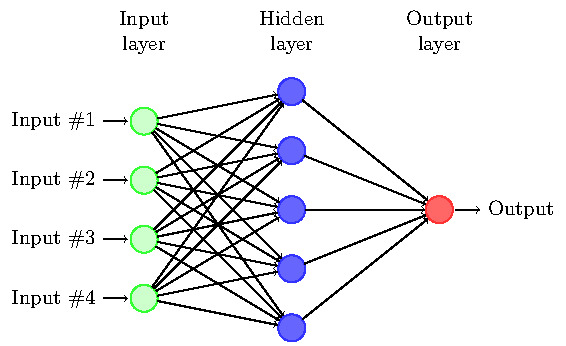
\includegraphics[width=0.6\textwidth]{FNN}
    \caption{前向神经网络结构}
    \label{fig:FNN}
\end{figure}

将多个神经元按层排列,各层之间前后级联,就组成了前向神经网络(Feedforward neural network, FNN),其结构如图~\ref{fig:FNN}所示。前向神经网络通常包含了输入层、隐藏层和输出层。

卷积神经网络(Convolutional Neural Network, CNN)是目前最常用的一种前向神经网络,对于大型图像处理有出色表现。一个典型的卷积神经网络结构(LeNet-5)\citep{lecun1998gradient} 如图~\ref{fig:CNN}所示:

\begin{figure}[!htbp]
    \centering
    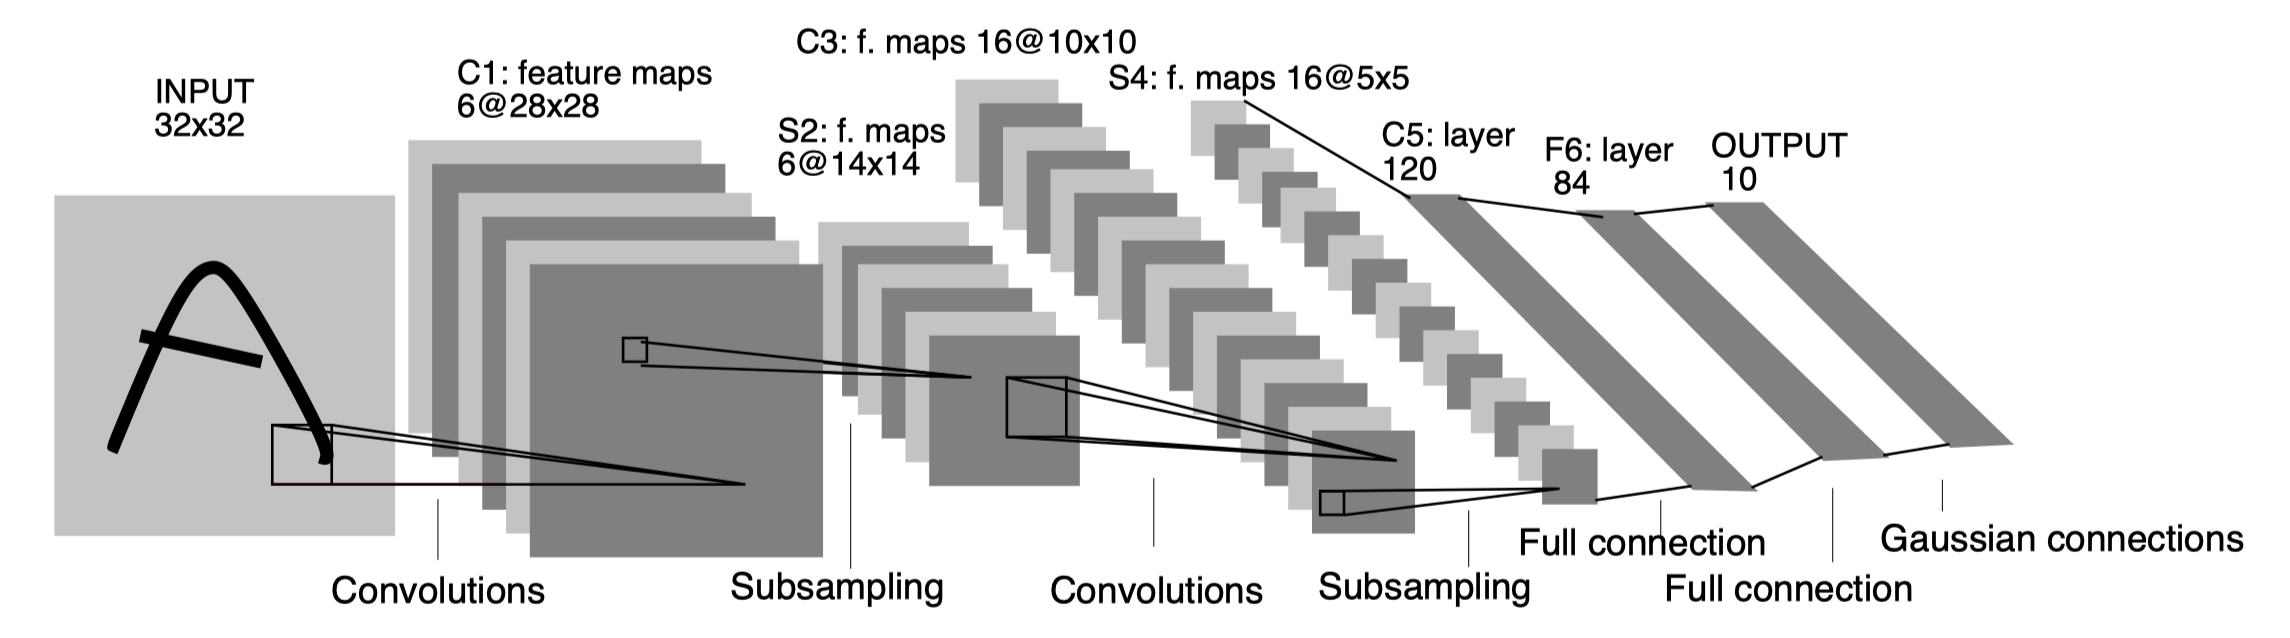
\includegraphics[width=0.9\textwidth]{CNN}
    \caption{LeNet-5 \ 网络结构}
    \label{fig:CNN}
\end{figure}

输入为一幅手写字母的图像,经过卷积神经网络的运算后,输出识别的结果。卷积神经网络主要包含了卷积层、池化层和全连接层 3 种结构,卷积层主要用来提取图像中的局部特征,池化层用来降低参数数量级,全连接层类似于卷积层,用来输出结果。

\subsection{YOLO 算法介绍}

YOLO 算法\citep{redmon2016you}于2016由 Joseph Redmon 等人提出,YOLO 的全称是 you only look once,指只需要浏览一次就可以识别出图像中物体的类别和位置。相比于 Region-based 的两阶段(2-stage)方式,YOLO 的单阶段(1-stage)扫描方式更适合通过流水线优化的方法进行硬件加速。YOLO 算法目前已经发展到了第四代,但是由于 YOLO V3 和 YOLO V4 引入了残差模型和FPN架构等新结构,使得整个神经网络结构更深,从 YOLO V2 的 darknet-19\citep{redmon2017yolo9000} 到 YOLO V3 的 darknet-53\citep{redmon2018yolov3},通过硬件加速需要消耗更多的资源,在低成本的 FPGA 芯片上难以实现,因此本文选用了 YOLO V2 算法作为硬件加速的对象。

TINY YOLO 算法是 YOLO 算法的简化版,在牺牲一定精度的代价下,其速度得到了大幅提高,且结构更加精简,适得其更加适合在硬件资源极度有限的低成本 FPGA 上实现。TINY YOLO 算法与 YOLO 算法的对比见表~\ref{tab:tiny},可以看到,对比原版 YOLO 算法,TINY YOLO 算法在准确度上有小幅度下降,但是其速度极快,最快达到了 207 FPS。

\begin{table}[!htbp]
\caption{TINY YOLO 与 YOLO 对比}
\label{tab:tiny}
\centering
\footnotesize% fontsize
\setlength{\tabcolsep}{4pt}% column separation
\renewcommand{\arraystretch}{1.2}%row space 
\begin{tabular}{lccccc}
\toprule
Model & Train & Test & mAP & FLOPS & FPS \\
\midrule
YOLOv2 & VOC 2007+2012 & 2007 & 76.8 & 34.90 Bn & 67 \\
YOLOv2 544x544 & VOC 2007+2012 & 2007 & 78.6 & 59.68 Bn & 40 \\
Tiny YOLO & VOC 2007+2012 & 2007 & 57.1 & 6.97 Bn & 207 \\
\bottomrule
\end{tabular}
\end{table}

YOLO V2 算法的结构如表~\ref{tab:darknet19}所示,其包含了19个卷积层,5个最大池化层以及一个全连接层。

% \begin{figure}[!htbp]
%     \centering
%     \includegraphics[height=0.70\textheight]{yolov2-tiny-structure}
%     \caption{TINY YOLO 网络结构}
%     \label{fig:yolov2-tiny-structure}
% \end{figure}


% \begin{table}[!htbp]
% \caption{Darknet-19}
% \label{tab:darknet19}
% \centering
% \footnotesize% fontsize
% \setlength{\tabcolsep}{4pt}% column separation
% \renewcommand{\arraystretch}{1.0}%row space 
% \begin{tabular}{c|c|c|c}
% \toprule
% Type & Filters & Size/Stride & Output \\
% \midrule
% Convolutional & 32   & 3 × 3   & 224 × 224 \\
% Maxpool       &      & 2 × 2/2 & 112 × 112 \\
% Convolutional & 64   & 3 × 3   & 112 × 112 \\
% Maxpool       &      & 2 × 2/2 & 56 × 56 \\
% Convolutional & 128  & 3 × 3   & 56 × 56 \\
% Convolutional & 64   & 1 × 1   & 56 × 56 \\
% Convolutional & 128  & 3 × 3   & 56 × 56 \\
% Maxpool       &      & 2 × 2/2 & 28 × 28 \\
% Convolutional & 256  & 3 × 3   & 28 × 28 \\
% Convolutional & 128  & 1 × 1   & 28 × 28 \\
% Convolutional & 256  & 3 × 3   & 28 × 28 \\
% Maxpool       &      & 2 × 2/2 & 14 × 14 \\
% Convolutional & 512  & 3 × 3   & 14 × 14 \\
% Convolutional & 256  & 1 × 1   & 14 × 14 \\
% Convolutional & 512  & 3 × 3   & 14 × 14 \\
% Convolutional & 256  & 1 × 1   & 14 × 14 \\
% Convolutional & 512  & 3 × 3   & 14 × 14 \\
% Maxpool       &      & 2 × 2/2 & 7 × 7 \\
% Convolutional & 1024 & 3 × 3   & 7 × 7 \\
% Convolutional & 512  & 1 × 1   & 7 × 7 \\
% Convolutional & 1024 & 3 × 3   & 7 × 7 \\
% Convolutional & 512  & 1 × 1   & 7 × 7 \\
% Convolutional & 1024 & 3 × 3   & 7 × 7 \\
% \midrule

% Convolutional & 1000 & 1 × 1   & 7 × 7 \\
% Avgpool       &      & Global  & 1000 \\
% Softmax       &      &         &      \\
% \bottomrule
% \end{tabular}
% \end{table}

{
\zihao{-5}
% Change the intercolumn space
\setlength{\tabcolsep}{10pt}

\begin{longtable}{cccc}
    \caption{Darknet-19 网络结构} \label{tab:darknet19}\\

    % Appear table header at the first page as well
    \toprule
    Type & Filters & Size/Stride & Output \\
    \midrule
    \endfirsthead

    \multicolumn{4}{c}%
    {\bfseries\small \tablename\ \thetable\ {续表}}\\

    % Appear the table header at the top of every page
    \toprule
    Type & Filters & Size/Stride & Output \\
    \midrule
    \endhead

    \midrule \multicolumn{4}{r}{\textit{续表见下页}}\\
    \endfoot

     % Appear \hline at the bottom of every page
    \bottomrule
    \endlastfoot

    Convolutional & 32   & 3 × 3   & 224 × 224 \\
    Maxpool       &      & 2 × 2/2 & 112 × 112 \\
    Convolutional & 64   & 3 × 3   & 112 × 112 \\
    Maxpool       &      & 2 × 2/2 & 56 × 56 \\
    Convolutional & 128  & 3 × 3   & 56 × 56 \\
    Convolutional & 64   & 1 × 1   & 56 × 56 \\
    Convolutional & 128  & 3 × 3   & 56 × 56 \\
    Maxpool       &      & 2 × 2/2 & 28 × 28 \\
    Convolutional & 256  & 3 × 3   & 28 × 28 \\
    Convolutional & 128  & 1 × 1   & 28 × 28 \\
    Convolutional & 256  & 3 × 3   & 28 × 28 \\
    Maxpool       &      & 2 × 2/2 & 14 × 14 \\
    Convolutional & 512  & 3 × 3   & 14 × 14 \\
    Convolutional & 256  & 1 × 1   & 14 × 14 \\
    Convolutional & 512  & 3 × 3   & 14 × 14 \\
    Convolutional & 256  & 1 × 1   & 14 × 14 \\
    Convolutional & 512  & 3 × 3   & 14 × 14 \\
    Maxpool       &      & 2 × 2/2 & 7 × 7 \\
    Convolutional & 1024 & 3 × 3   & 7 × 7 \\
    Convolutional & 512  & 1 × 1   & 7 × 7 \\
    Convolutional & 1024 & 3 × 3   & 7 × 7 \\
    Convolutional & 512  & 1 × 1   & 7 × 7 \\
    Convolutional & 1024 & 3 × 3   & 7 × 7 \\
    \midrule

    Convolutional & 1000 & 1 × 1   & 7 × 7 \\
    Avgpool       &      & Global  & 1000 \\
    Softmax       &      &         &      \\
\end{longtable}
}

根据 YOLO 论文\citep{redmon2016you,redmon2017yolo9000,redmon2018yolov3}及 Darknet 网络源码分析 YOLO V2 进行目标检测的步骤如下:

\begin{enumerate}
\item 首先输入任意尺寸的 RGB 格式的图像,将各像素的值归一化到0-1之间,再将图像进行缩放到 $244 \times 244$ 大小,不改变图像的比例,不足处用 0.5 补充,这样就得到了 $244 \times 244 \times 3$ 的矩阵;
\item 将(1)中得到的矩阵输入 Darknet 网络进行检测,网络检测后输出 $7 \times 7 \times 1024$ 的矩阵;
\item 对网络输出的结果进行处理,获取输出的边框的信息,再根据各个边框的位置,可信度等,获得最有可能的边框位置。
\end{enumerate}

\section{RISC-V 概述}
RISC-V 是由加州大学伯克利分校( UCB )提出的一种开源精简指令集架构(Instruction Set Architecture, ISA)\citep{waterman2011risc},目前已经有了一个完整的硬件和硬件生态\citep{asanovic2014instruction},包括完整的指令集、相应的编译器、模拟器和工具链。利用开源的RISC-V处理器,研究人员可以方便地将可重构加速器整合进 SOC,并拓展相应的指令集来实现加速器的软件接口。

\section{FPGA技术概述}

\subsection{FPGA 介绍}

FPGA 的全称为现场可编程逻辑门阵列(Field Programmable Gate Array, FPGA),是一种半定制的集成电路(Integrated Circuit, IC)芯片。FPGA 包含了一组可编程逻辑门阵列(Programmable Logic Blocks, PLB)以及可重配置的互联层次结构,通过这种结构可以将 PLB 连接在一起。FPGA 可以通过重编程,实现不同逻辑特性,从而实现了可重构计算。因此理论上 FPGA 可以实现当前 CPU 上的所有算法,但是具体算法实现的效果会受制于 FPGA 的可用资源、时钟频率以及输入输出的带宽。

\subsection{AXI4 总线协议}

在 Xilinx 的设计工具中提供的 IP 核大多使用 AXI4 总线来实现各级之间的逻辑控制和数据传输。为了保证本设计中 SOC 的通用性,提高设计效率,因此使用 AXI4 总线作为 SOC 的片内总线,为此这里对 AXI4 总线做详细介绍。

AXI4(Advanced eXtensible Interface)总线是由 ARM 公司提出的AMBA(Advanced Microcontroller Bus Architecture)协议中的一部分,Xilinx 公司在其基础上又发展出了 AXI Lite 和 AXI Stream 两种简化接口。因此目前 Xilinx 的 IP 中主要使用了 AXI Full、AXI Stream 和 AXI Lite 三种接口。在本设计中主要使用到的是 AXI Full 和 AXI Lite 总线。
% ,下面对其分别说明。

% \subsubsection{AXI Full}

% \subsubsection{AXI Lite}

\section{本章小结}

本章主要介绍的在设计过程中涉及到相关技术,包括了卷积神经网络、RISC-V 处理器、FPGA 等。其中在卷积神经网络介绍部分,对 YOLO V2 算法进行了详细的说明。由于在 SOC 设计的过程中,AXI4 总线也被大量使用,关系到 SOC 内部以及 CNN 加速器的效果,因此也对其进行了详细的介绍。
